% -------------------------------------------------------------------------------------------------
% Definitionen
% -------------------------------------------------------------------------------------------------
\documentclass[
    fontsize=12pt,                      % Schriftgröße 12 pt
    paper=a4,                           % Seitengröße A4
    twoside=off,                       % zweiseitiger Druck
    DIV=15,                             % Seiteneinteilung
    BCOR=12mm,                          % Bindekorrektur
    headings=normal,                    % normal große Überschriften
    headsepline=false,                   % Trennlinie unter der Kopfzeile
    footsepline=false,                  % Trennlinie über der Fußzeile
    headinclude=true,                   % Kopfzeile zählt zum Textkörper
    footinclude=false,                  % Fußzeile zählt nicht zum Textkörper
    toc=listof,                         % Verzeichnisse der Gleitumgebungen ins Inhaltsverzeichnis
    toc=bib,                            % Literaturverzeichnis ins Inhaltsverzeichnis
    chapterprefix=false,                % vor Kapitelnummern steht "Kapitel"
    appendixprefix=false,               % vor Anhangüberschriften steht "Anhang"
    numbers=noendperiod,                % Keinen Punkt hinter die letzte Zahl eines Kapitels (auch bei Anhang)
    captions=tableabove,                % Tabellenüberschriften setzen
    footnotes=multiple,                 % Erkennung von mehreren Fußnoten hintereinander
    bibliography=oldstyle,              % Literaturverzeichnis: openstyle oder oldstyle
    draft=false,                        % Entwurfsstadium
]{scrreprt}


% Paket Includes
% ----------------------------
\usepackage[T1]{fontenc}                % deutsche Umlaute und Sonderzeichen
\usepackage[utf8]{inputenc}             % Umlaute koennen direkt im Quelltext stehen
\usepackage[ngerman]{babel}             % neue deutsche Rechtschreibung 
\usepackage{lmodern}
\usepackage{graphicx}                   % Bilder einfügen
\usepackage{tabularx}                   % Tabellen mit fester Breite und variabler Spaltenbreite
\usepackage{array,longtable}            % Tabellen mit Seitenumbruch
\usepackage{booktabs}                   % bessere horizontale Linien in Tabellen
\usepackage{array,ragged2e}             % mehr Spaltentypen in Tabellen und neue Spaltentypen
\usepackage{dcolumn}                    % Spalten am Dezimaltrenner ausrichten
\usepackage{amsmath}
\usepackage[                            % Unterabbildungen mit folgenden Parametern:
            font=footnotesize,          % kleine Schrift
            labelfont={sf,bf},          % Labels fett und serifenlos
            textfont={sf},              % Text serifenlos
            format=hang,                % hängender Einzug
           ]{caption}
\usepackage{float}      
\usepackage{hyperref}                   % URL links     
\usepackage{xcolor} 
\usepackage{listings}
\usepackage{subfig}

\definecolor{myblue}{rgb}{0,0.3137,0.5843}
\definecolor{mygreen}{rgb}{0,0.6,0}
\definecolor{myred}{rgb}{0.7529,0.3137,0.3019}

\newcommand{\Farbcode}[1]{\texttt{\textbf{\textcolor{myred}{#1}}}}


% Kopf- und Fußzeile
% ----------------------------
\usepackage{scrlayer-scrpage} 
\setkomafont{pagehead}{\sffamily\small}
\setkomafont{pagefoot}{\sffamily\small}
%\automark{chapter}
\lohead{Modul Embedded Systems 2 – Steuergeräte, Vernetzung, Software} \cohead{} \rohead{Übung 1-4}
\lofoot{\includegraphics[height=10pt]{Figures/HSMW-Logo-klein} HS Mittweida, INW, Prof. Thomanek}
\cofoot{} \rofoot{\thepage}

\pagestyle{headings}
\renewcommand*{\chapterpagestyle}{headings}% Nicht zu empfehlen, aber du willst das offenbar trotzdem.


\setcounter{secnumdepth} {3}
\addto\captionsngerman{\renewcommand{\figurename}{Abb.}}    % Verwende Abb. x.x anstatt Abbildung x.x
\renewcommand{\thefigure}{\arabic{figure}}
% -------------------------------------------------------------------------------------------------
% Dokument
% -------------------------------------------------------------------------------------------------

\begin{document}


\chapter*{Übung 1-4 -- Übermitteln von CAN-Daten}

Über einen \text{Thermistor} (Heißleiter, NTC (MF52-103 3435)) soll die Temperatur gemessen werden. Dabei wird der Spannungsabfall über den temperaturabhängigen Widerstand mithilfe eines Spannungsteilers gemessen.

\vskip 0.2cm
\noindent

Die gemessene Temperatur soll auf dem \textbf{CAN übertragen} werden. Dafür wird der Mikrokontroller \textbf{Aurix TC374} verwendet, der eine integrierte CAN-Schnittstelle bietet. Der \textbf{CAN-Transceiver „TLE9251VSJ“} von Infineon ist auf dem TC375 verbaut.

\vskip 0.2cm
\noindent

% Die Kommunikation mit dem CAN-Bus erfolgt über den Anschluss an die Pins CAN-H und CAN-L des Mikrokontrollers, wie in der Abbildung dargestellt.

\vskip 0.5cm
\section*{Schaltungsaufbau} 
\begin{itemize}
\item Spannungsteiler: Vorwiderstand (10~k$\Omega$) an 5V und NTC (10~k$\Omega$ bei $25^\circ$C) an Masse
\item Spannungsabgriff an Eingang A5 des Aurix TC375 mit einer Auflösung des ADC von 10~Bit bei Spannungsbereich von 0 \dots 5V
\end{itemize}

\begin{figure}[H]
  \centering
  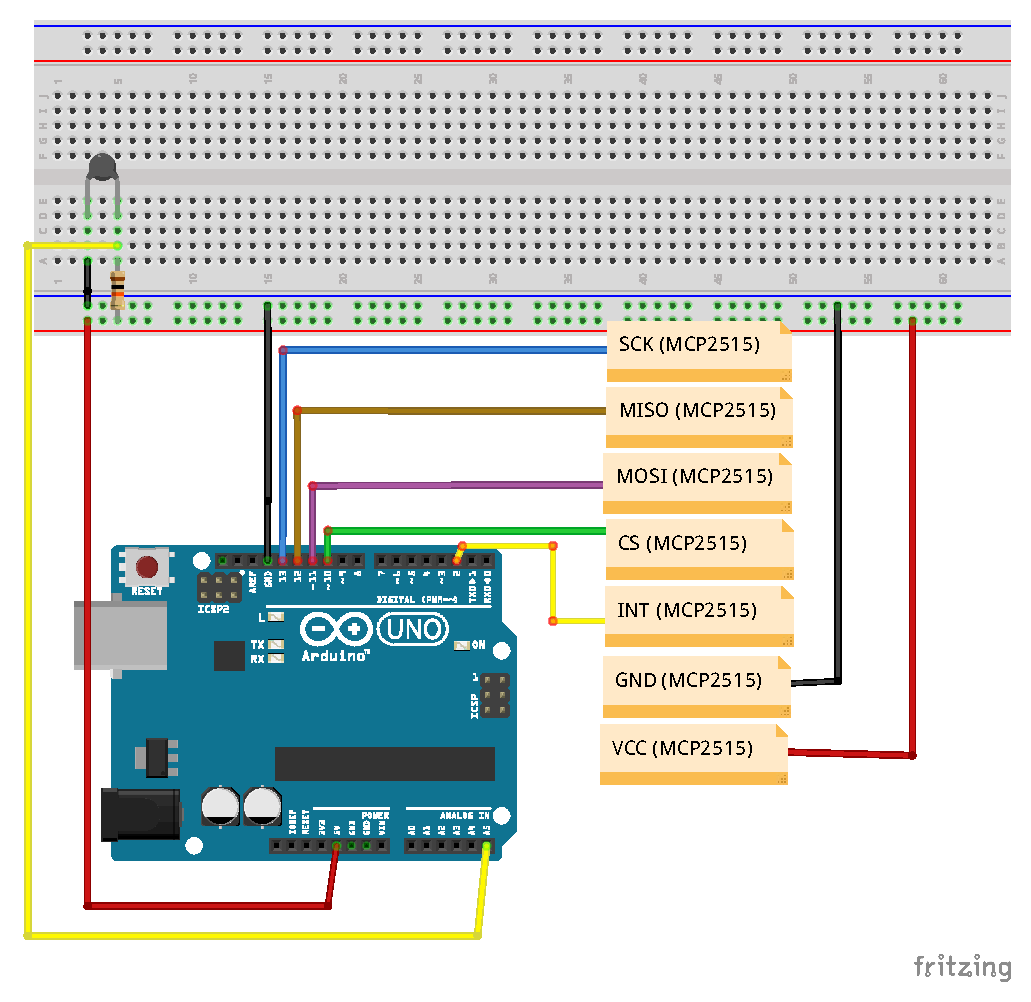
\includegraphics[width=0.45\linewidth]{Fritzing/Uebung_104_Steckplatine}
  \caption{Steckplatine}
\end{figure}

\section*{Softwareerstellung} 

Verwenden Sie als Basis das Aurix-Development-Studio-Template \Farbcode{Uebung\_104\_Template.zip}. Importieren sie das Projekt Erstellen Sie einen \textbf{Ordner} mit dem Name \Farbcode{Can} und legen Sie in diesem Ordner die aus OPAL heruntergeladenen \textbf{vier Dateien} (\Farbcode{can.ino}, \Farbcode{can.h}, \Farbcode{mcp2515.h}, \Farbcode{mcp2515.cpp}) ab.

Für weitere Hilfe bei der Programmierung mittel Arduino-Bibliothek siehe  \url{https://www.arduino.cc/reference/de/} sowie zum MCP2515-Treiber im Anhang dieser Anleitung.
\vskip 0.2cm

\noindent
\textbf{Initialisierung:} ( \Farbcode{void setup()} )
\begin{itemize}
\item Initialisierung der CAN-Nachricht (Länge, CAN-ID, ...) \\
\textbf{Beachte:} Der CAN-ID lautet 100h + <Testplatznummer> -- Somit sendet bspw. der Testplatz 4 seine Temperatur unter der CAN-ID \texttt{\textbf{104h}} und der Testplatz 10 mit der ID \texttt{\textbf{10Ah}}
\item Initialisierung des CAN-Controllers mittels \Farbcode{mcp2515.reset()}
\item Setzen der Bitrate auf 500~kBit/s und Taktfrequenz 8~MHz mittels \\ \Farbcode{mcp2515.setBitrate(...)}
\item Aktivieren des Normal-Modes mittels \Farbcode{mcp2515.setNormalMode()}
\item Serielle Konsole für Debug-Zwecke aktivieren mittels \Farbcode{Serial.begin(9600)}
\end{itemize}

\noindent
\textbf{Endlosschleife:} ( \Farbcode{void loop()} )
\begin{enumerate}
\item Spannungswert am Pin A5 mittels \Farbcode{analogRead()} einlesen und in Spannung umwandeln
\item Widerstand des Thermistors anhand Spannungsteilerregel bestimmen
\item Temperatur aus Widerstandswert bestimmen gemäß Formel
\begin{equation*}
T(R)=\frac{1}{\frac{1}{B}\ln(\frac{R}{R_{25}})+\frac{1}{T_{25}}} 
\end{equation*}
wobei $B$ -- Sensorkonstante, $R_{25}$ -- Widerstand des Thermistors bei $25^\circ$C, $T_{25}$ -- Temperatur in Kelvin ($25^\circ$C)

Ermitteln Sie die Sensorkonstante (B-Wert) aus dem Datenblatt des Thermistors (Siehe OPAL).
\item Ausgeben des Temperaturwert auf der seriellen Konsole und Kopieren in eine CAN-Botschaft \\
\textbf{Beachte:} Auf dem AVR µC werden float-Variablen im Little-Endian-Format abgelegt -- auch die erstellte CAN-Datenbasis erwartet die Temperatur in der CAN-Nachricht im Little-Endian-Format

\item Die Übertragung der Temperatur soll zyklisch aller 1000 ms erfolgen
\end{enumerate}
\newpage
\section*{Anhang -- Infos zum MCP2515-Treiber} 
\noindent
\textbf{CAN-Nachricht-Format:} (siehe  \Farbcode{can.h})
\lstset{language=C++,
	basicstyle=\small\ttfamily,  
	commentstyle=\color{mygreen},
	showstringspaces=false,
	keywordstyle=\color{blue},
	breakatwhitespace=false,        
	breaklines=true}
\begin{lstlisting}[frame=single,  label=LST_MyCam]
struct can_frame {
    canid_t can_id;  /* 32 bit CAN_ID + EFF/RTR/ERR flags */
    __u8    can_dlc; /* frame payload length in byte  */
    __u8    data[CAN_MAX_DLEN] __attribute__((aligned(8)));
};
\end{lstlisting}
\vskip 0.5cm
\noindent
\textbf{Notwendige Methoden des MCP2515-Treibers:} (siehe \Farbcode{mcp2515.h})
\begin{lstlisting}[frame=single,  label=LST_MyCam]
 // Konstruktor
 MCP2515(const uint8_t _CS, 
         const uint32_t _SPI_CLOCK = DEFAULT_SPI_CLOCK);
 // Reset
 ERROR reset(void);
 // Set to Normal Mode
 ERROR setNormalMode();
 // Set Bitrate and Clock Frequency
 ERROR setBitrate(const CAN_SPEED canSpeed, const CAN_CLOCK canClock);
 // Send a message
 ERROR sendMessage(const struct can_frame *frame);
\end{lstlisting}
\vskip 0.5cm
\noindent
\textbf{Mögliche Taktfrequenzen:} (siehe \Farbcode{mcp2515.h})
\begin{lstlisting}[frame=single,  label=LST_MyCam]
enum CAN_CLOCK {
  MCP_20MHZ,
  MCP_16MHZ,
  MCP_8MHZ
};
\end{lstlisting}
\vskip 0.5cm
\noindent
\textbf{Mögliche CAN-Bitraten:} (siehe \Farbcode{mcp2515.h})
\begin{lstlisting}[frame=single,  label=LST_MyCam]
enum CAN_SPEED {
  CAN_5KBPS,
  CAN_10KBPS,
  CAN_20KBPS,
  ...
  CAN_100KBPS,
  CAN_125KBPS,
  CAN_200KBPS,
  CAN_250KBPS,
  CAN_500KBPS,
  CAN_1000KBPS
};
\end{lstlisting}
\vskip 0.5cm
\noindent
\textbf{Fehlercodes:} (siehe \Farbcode{mcp2515.h})
\begin{lstlisting}[frame=single,  label=LST_MyCam]
class MCP2515
{
public:
  enum ERROR {
    ERROR_OK        = 0,
    ERROR_FAIL      = 1,
    ERROR_ALLTXBUSY = 2,
    ERROR_FAILINIT  = 3,
    ERROR_FAILTX    = 4,
    ERROR_NOMSG     = 5
  };
  ...
};  
\end{lstlisting}
\end{document}


